\chapter{Especificação e Modelagem de Sistemas Orientados a Aspectos}

Este capítulo apresenta um Perfil UML para especificação de sistemas orientados a aspectos e uma ferramenta para realizar a composição de interesses
núcleo com interesses entrecortantes (aspectos). O perfil UML fornece subsídios para realizar a modelagem e a composição automática de modelos núcleo
com modelos entrecortantes. A ferramenta que realiza a composição de modelos, o algoritmo e o visualizador de aspectos são apresentados na parte
final deste capítulo.

\section{Especificação de Sistemas Orientados a Aspectos}

O meta-modelo padrão da UML não permite a especificação de todas as características de sistemas orientados a aspectos. Este trabalho define um perfil
UML que estende a linguagem com novas construções, permitindo a modelagem de sistemas que utilizam aspectos. Esta seção descreve os
estereótipos, valores rotulados e restrições propostas por este perfil e também apresenta uma abordagem para representação das características estruturais e
comportamentais de aspectos, fornecendo subsídios para composição automática de modelos de aspectos com modelos núcleo do sistema. A figura
\ref{fig:uml_profile} apresenta o perfil UML proposto para representar a estrutura e o comportamento de aplicações orientadas a aspectos.
Este perfil pode ser utilizado em ferramentas CASE que suportem a importação de perfis através do padrão XML Metadata Interchange (XMI) \cite{xmi:11} para
troca de meta-dados via Extensible Markup Language (XML). 

\subsection{Especificação Estrutural}

Para modelagem estrutural, este trabalho utiliza algumas definições do trabalho proposto por Evermann \cite{Evermann:2007:MSP:1229375.1229379}, o qual
permite a representação das características estruturais de aspectos. As definições usadas do perfil de Evermann são os 
estereótipos \textit{CrosscuttingConcern} e \textit{Aspect}, que estão com o fundo bege no diagrama de perfil da figura
\ref{fig:uml_profile}. Um estereótipo estende um elemento do meta-modelo da UML, adicionando uma nova semântica a um elemento do modelo. Neste
trabalho, um elemento do meta-modelo a ser estendido é representado dentro de parênteses. O estereótipo \textit{CrosscuttingConcern} estende
(\textit{Package}) e contém um conjunto de classes e aspectos, representando um interesse que impacta uma ou mais partes de um sistema. O estereótipo
\textit{Aspect} estende (\textit{Class}), contém declarações inter-tipos (introduções) e algumas propriedades de configuração, que são valores
rotulados. O primeiro valor rotulado é \textit{isPrivileged} que determina se um aspecto é privilegiado, isto é, se ele tem acesso a membros privados
de outras classes do sistema. Outra propriedade que pode ser configurada é o tipo de instancialização de um aspecto. O tipo de instancialização é
definido pelos valores rotulados \textit{perType} e \textit{perPointcut}. O valor rotulado \textit{perType} é um enumerável com quatro opções:
\textit{perthis}, \textit{pertarget}, \textit{percflow}, \textit{percflowbelow} e define o tipo de instancialização. O valor
rotulado \textit{perPointcut} define qual é o ponto de corte que está associado. Um exemplo de uso desta variável seria a instanciação do aspecto para
cada fluxo de execução após a captura de um ponto de corte. Esta instanciação poderia incluir o próprio ponto de corte (\textit{percflow}), ou não (\textit{percflowbelow}). 

As declarações inter-tipos permitem a injeção de membros (métodos, atributos) em uma classe, mudanças de hierarchia de herança entre classes e de
implementação de interfaces. Para representar declarações inter-tipos, foi proposto o estereótipo \textit{ClassExtension}. Este estereótipo estende (\textit{Class}) e
está associado a outro estereótipo denominado \textit{Introduction}. O estereótipo \textit{Introduction} é usado para marcar quais membros estão sendo
inseridos em uma classe, ou qual relacionamento de herança está sendo adicionado ou removido, ou qual interface está sendo implementada. O estereótipo
\textit{Introduction} estende os elementos do meta-modelo (\textit{Attribute}), (\textit{Operation}), (\textit{Generalization}) e
(\textit{Realization}).

\begin{figure}[!h] \centering
	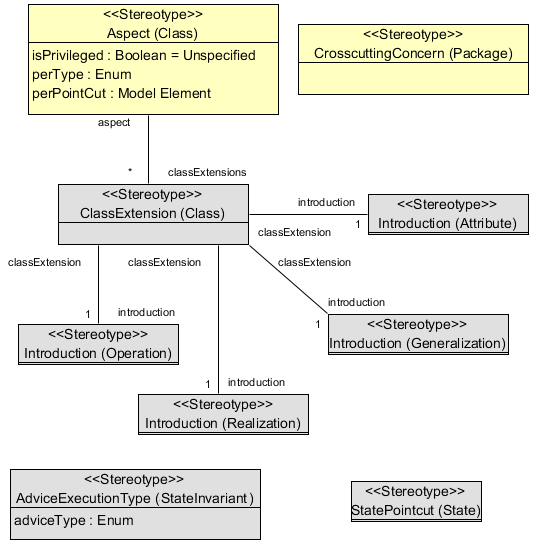
\includegraphics{img/full_profile.png}
	\caption{Perfil UML para Modelagem de Sistemas Orientados a Aspectos.}\label{fig:uml_profile}
\end{figure}

Com os estereótipos propostos e o diagrama de classes da UML é possível representar a estrutura de aplicações orientadas a aspectos usando
pacotes, classes e aspectos. O exemplo da figura \ref{fig:structural_profile_example} mostra como modelar um interesse entrecortante usando o perfil
UML proposto por esta dissertação. Alguns dos exemplos apresentados são baseados no sistema de gerenciamento de hotéis proposto por Jacobson para
apresentar sua proposta de modelagem \cite{Jacobson:2004:ASD:1062430}. O interesse sendo modelado é a capacidade de um objeto ter seu estado copiado
para outro objeto. A funcionalidade \textit{Copyable} é especificada como um interesse entrecortante que contém o aspecto
\textit{CopyableAspect}, duas extensões de classes e a definição da interface \textit{ICopyable}. As classes \textit{Room} e \textit{Reservation}
são marcadas com o estereótipo \textit{ClassExtension}, para sinalizar que estão sendo estendidas pelo aspecto. A primeira extensão adicionada as
classes é a implementação da interface \textit{ICopyable}, que define dois métodos para um objeto ter a capacidade de ser copiável. Como a interface
\textit{ICopyable} exige a implementação de dois métodos, o aspecto introduz os métodos \textit{copy()} e \textit{deepCopy()} nas classes \textit{Room} e \textit{Reservation}. 
A realização da interface \textit{ICopyable} em ambas as classes e os métodos introduzidos são marcados com o estereótipo \textit{Introduction}.

\begin{figure}[!h] \centering
	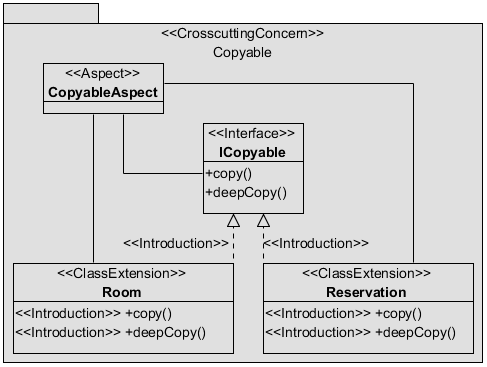
\includegraphics{img/structural_profile_example.png}
	\caption{Exemplo de Modelagem Estrutural: Interesse Entrecortante \textit{Copyable}.}\label{fig:structural_profile_example}
\end{figure}

\subsection{Especificação Comportamental}

Além da especificação estrutural, com declarações inter=tipos e configurações de instancialização, deve-se especificar o comportamento de um aspecto.
Um aspecto é composto por pontos de corte e avisos, os quais definem em quais pontos e qual comportamento estenderá um sistema. O perfil de Evermann 
\cite{Evermann:2007:MSP:1229375.1229379} representa pontos de corte dentro da própria especificação de aspecto, isto é, na representação estrutural de
um aspecto com classes. Esta forma de especificação não permite a captura de múltiplos pontos de junção em um mesmo ponto de corte, pois
apenas outros elementos do modelo UML podem ser selecionados. A abordagem proposta nesta dissertação representa pontos de corte com o diagrama de máquina 
de estados da UML. Cada transição representa a captura de um ou mais pontos de junção, com a possibilidade de uso de expressões regulares
(\textit{wildcards}) para captura de múltiplos pontos de execução em uma mesma construção. Se a captura de todos os pontos de junção for 
satisfeita, isto é, se as condições para disparar uma transição forem satisfeitas, considera-se que o sistema satisfez um ponto de corte. A composição
de pontos de corte é realizada através da composição de diferentes máquinas de estado. No perfil proposto, o estereótipo \textit{StatePointcut} 
estende (\textit{State}) e representa um ponto de corte. A definição deste estereótipo pode ser visualizada na figura \ref{fig:uml_profile}.

A figura \ref{fig:pointcut_definition_1} mostra um exemplo de definição de um ponto de corte. O ponto de corte \textit{AnyCall} captura chamadas
(ponto de corte do tipo \textit{call}) a qualquer método, de qualquer classe, usando uma expressão regular (\textit{wildcard}) para capturar qualquer
tipo de retorno, qualquer classe e qualquer nome de método com qualquer número de parâmetros. O ponto de corte \textit{RoomTarget} captura a ocorrência de uma chamada
quando o objeto alvo (ponto de corte do tipo \textit{target}) é do tipo \textit{Room}. Cada ponto de corte é representado como um estado no diagrama
de máquina de estados. A assinatura de um ponto de corte é especificada na transição que leva ao estado do ponto de corte, a qual permite o uso de
\textit{wildcards} para capturar múltiplos pontos de junção. Quando um ponto de corte é satisfeito, significa que o sistema capturou os pontos de execução 
especificados pela assinatura do ponto de corte.

\begin{figure}[h]
	\centering
	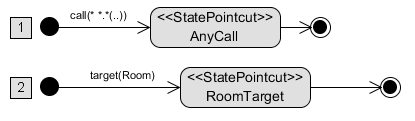
\includegraphics{img/pointcut_definition_1.png}
	\caption{Definição de Dois Pontos de Corte.}\label{fig:pointcut_definition_1}
\end{figure}

A linguagem AspectJ permite a composição de pontos de corte com os operadores lógicos \textit{and} e \textit{or}. A abordagem proposta nesta
dissertação realiza a composição automática de pontos de corte usando o diagrama de máquina de estados. Os próximos exemplos apresentam a composição
de pontos de corte proposta por esta dissertação. A figura \ref{fig:pointcut_definition_and} apresenta a composição dos pontos de corte
\textit{AnyCall} e \textit{RoomTarget} usando o operator \textit{and}. A máquina de estado composta contém um estado com uma região concorrent, contendo 
sub-estados que executam concorrentemente: \textit{AnyCall} e \textit{RoomTarget}. A sincronização ocorre com os nodos \textit{fork} e \textit{join}, 
os quais garantem que o estado final (\textit{AnyCall AND RoomTarget}) somente será satisfeito se ambos os estados (\textit{AnyCall} e \textit{RoomTarget} 
forem satisfeitos. Esta é a semântica do operador \textit{and} na linguagem AspectJ. A figura
\ref{fig:pointcut_definition_or} apresenta a composição de pontos de corte usando o operador \textit{or}. Neste caso a semântica é um pouco diferente,
porque o sistema alcançara o estado final (\textit{AnyCall OR RoomTarget}) quando qualquer um dos pontos de corte for satisfeito. Este comportamento é
representado na máquina de estados composto, que contém transições diretas de ambos estados para o estado final.

\begin{figure}[h]
	\centering
	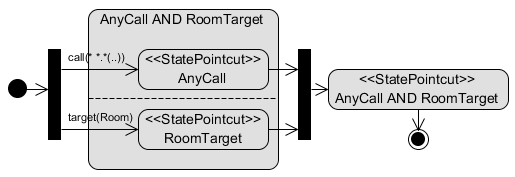
\includegraphics{img/pointcut_definition_and.png}
	\caption{A composição de dois pontos de corte com o operador AND.}\label{fig:pointcut_definition_and}
\end{figure}

\begin{figure}[h]
	\centering
	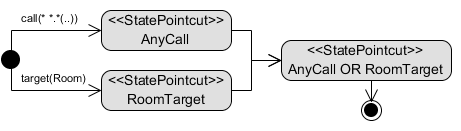
\includegraphics{img/pointcut_definition_or.png}
	\caption{A composição de dois pontos de corte com o operador OR.}\label{fig:pointcut_definition_or}
\end{figure}

Um ponto de corte captura somente os pontos de execução de um sistema. O comportamento que deve ser injetado nestes pontos é representado pelo aviso,
o qual está diretamente associado a um ponto de corte. Diagramas de sequência são utilizados para representar o comportamento dos interesses núcleo
(modelo núcleo) e dos interesses entrecortantes (modelos entrecortantes). Um aspecto pode conter um ou mais avisos e cada um é representado por um
modelo entrecortante. O comportamento de um aviso executa quando os pontos de corte associados ao mesmo são satisfeitos, isto é, todos os pontos de
junção são capturados. Como nesta dissertação pontos de corte são modelados com o diagrama de máquina de estados e avisos com o diagrama de sequência,
a conexão entre avisos com pontos de corte deve ser realizada utilizando elementos sintáticos destes diagramas. A conexão entre estes elementos é
realizada através do uso de invariantes de estado. Uma invariante de estado é um fragmento de interação associado com a linha de vida de um diagrama
de sequência, representado uma restrição em tempo de execução nos participantes da interação. A alcançabilidade de um estado é usado como restrição
para disparar a execução de um aviso. 

A definição de um modelo entrecortante (como um diagrama de sequência) inicia adicionando o aspecto como o elemento associado a primeira linha de vida
do diagrama. Uma invariante de estado, a qual representa a satisfação do ponto de corte, é associada a linha de vida do aspecto. Isto significa que a
sequência de mensagens ocorrerá somente quando o sistema atingir o estado representado pela invariante de estado. As mensagens podem ser executados
antes, durante ou depois do disparo do ponto de corte. O tempo de execução das mensagens adicionadas pelo aspecto é configurado usando o estereótipo
\textit{AdviceExecutionType}. Este estereótipo estende (\textit{StateInvariant}) e é apresentado na parte inferior da figura \ref{fig:uml_profile}. O
estereótipo \textit{AdviceExecutionType} tem um valor rotulado do tipo enumeração denominado de \textit{adviceType}. Os tipos válidos para este enumerável são:
antes, durante ou depois.

A conexão entre avisos e pontos de corte pode ser melhor compreendida no exemplo da figura \ref{fig:behavioral_profile_example}. A figura
\ref{fig:behavioral_profile_example} apresenta o ponto de corte previamente especificado para captura de chamadas (ponto de corte \textit{call}) de
qualquer método em qualquer classe com qualquer número de parâmetros (\textit{AnyCall}). O aspecto de registro de mensagens (\textit{log}) define um
modelo entrecortante que registra uma mensagem usando uma classe do tipo \textit{Logger}. O modelo entrecortante é descrito como uma sequência de
mensagens em uma diagrama de sequência. Este diagrama contém uma invariante de estado que referencia o ponto de corte \textit{AnyCall}. Uma invariante
de estado deve ter o estereótipo \textit{AdviceExecutionType} e o valor rotulado \textit{adviceType} para especificar quando o comportamento do aviso
será executado. No exemplo, o comportamento do aspecto será eecutado depois (\textit{after}) dos pontos de junção capturados pelo ponto de corte
\textit{AnyCall}. A mensagem \textit{log()} será executada somente quando o estado \textit{AnyCall} for satisfeito.


\begin{figure}[h]
	\centering
	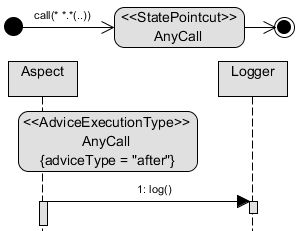
\includegraphics{img/behavioral_profile_example.png}
	\caption{A conexão entre pontos de corte e avisos usando invariantes de estado.}\label{fig:behavioral_profile_example}
\end{figure}

\section{Visualização e Composição Automatizada de Aspectos}

Esta seção apresenta a ferramenta \textit{SEA/Aspect} que é um dos produtos do esforço de pesquisa relatado nesta dissertação, a qual permite a
visualização de modelos entrecortantes compostos com modelos núcleo utilizando diagramas de classe e de sequência. O algoritmo para composição de 
modelos é descrito em passos para realizar a composição de classes e de mensagens. Finalmente, o visualizador de aspectos é apresentado.

\subsection{A Ferramenta SEA/Aspect}

O perfil UML proposto fornece subsídios para composição e visualização dinâmica de aspectos. O perfil foi adicionado no ambiente de desenvolvimento
SEA \cite{silva:00}, o qual suporta a diagramação e modelagem UML. A ferramenta SEA/Aspect permite a seleção de quais modelos entrecortantes serão
compostos com os modelos núcleo do sistema. Um desenvolvedor pode automaticamente visualizar somente os modelos núcleo, os modelos entrecortantes, ou
os modelos núcleo compotos com os entrecortantes. Aspectos podem ser habilitados ou desabilitados dinamicamente, atualizando o modelo composto. Esta
atualização automática permite a mudança de visões, visualizando diferentes composições de modelos.

A composição de modelos da ferramenta SEA/Aspect tem dois passos para produzir um modelo composto: \textbf{seleção} e \textbf{composição},
as quais são descritas nas próximas duas seções. A fase de seleção deve ser executada manualmente pelo desenvolvedor, enquanto a fase de composição é
executada automaticamente pelo algoritmo de composição do ambiente SEA.

\subsubsection{Seleção}
  
Nesta etapa o desenvolvedor seleciona manualmente quais modelos núcleo e entrecortantes deseja compor atribuindo uma cor diferente para cada modelo.
Estas cores diferenciam os elementos de cada modelo no modelo composto. As mensagens enviadas pelos objetos de cada modelo serão preenchidas com a cor
associada ao modelo em questão. A figura \ref{fig:selection_screen} apresenta a janela para seleção de aspectos na ferramenta SEA/Aspect. Neste
exemplo é possível visualizar três modelos entrecortantes: lista de espera (\textit{Waiting List}), registro de mensagens (\textit{Log}) e
programa de fidelidade (\textit{Earn Loyalty Points}) e um modelo núcleo: reserva de quarto (\textit{ReserveRoom}). Nesta seleção, o desenvolvedor
deseja visualizar a composição entre os modelos \textit{ReserveRoom}, \textit{Waiting List} e \textit{Log}.

  \begin{figure}[!h]
	\centering
	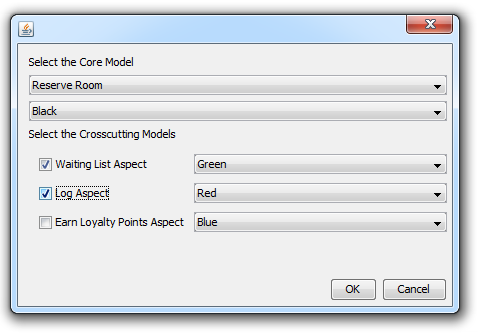
\includegraphics{img/selection_screen.png}
	\caption{Seleção de Modelos Para Composição.}\label{fig:selection_screen}
  \end{figure}
  
Os modelos núcleo e entrecortantes selecionados pelo desenvolvedor são utilizados como entrada da etapa de composição, que, basedo nos pontos de corte
e nas introduções dos modelos entrecortantes selecionará quais elementos devem ser modificados no modelo composto.  

\subsubsection{Composição}

A composição é realizada entre um modelo núcleo e um ou mais modelos entrecortantes, provendo como resultado um modelo composto com a estrutura ou o
comportamento dos modelos entrecortantes injetados no modelo núcleo. No modelo composto, o comportamento entrecortante diferencia-se do comportamento
núcleo pelas cores diferentes, como pode ser visualizado na figura \ref{fig:case_study_compound_2}, que mostra a composição de diagrama de
sequência entre os interesses de lista de espera, reserva de quarto e registro de mensagens de um sistema.

O meta-modelo do ambiente de desenvolvimento SEA \cite{silva:00} é utilizado para composição de modelos. Os principais elementos do meta-modelo podem ser
visualizados no diagrama da figura \ref{fig:sea_meta_model}. No meta-modelo do SEA, uma especificação (\textit{Specification}) agrega um conjunto de elementos de
especificação (\textit{SpecificationElement}), os quais podem ser modelos (\textit{ConceptualModel}) ou conceitos (\textit{Concept}). Estes modelos
de especificação podem ser associados com dois tipos de relacionamento: sustentabilidade (\textbf{sustainment}) e referência (\textbf{reference}). O
relacionamento de sustentabilidade estabelece uma relação semântica entre dois elementos, quando um assume o papel de sustentado e o outro de
sustentador. A semântica desse relacionamento é que o elemento sustentado existirá em uma especificação enquanto o elemento sustentador existir.
Um exemplo de relacionamento de sustentabilidade é o relacionamento entre classes, atributos e métodos, no qual uma classe é o sustentador e seus
campos são sustentados pela classe. O relacionamento de referência estabelece que elementos referenciadores dependem de um elemento referenciado. Um
exemplo deste tipo de relacionamento é uma mensagem em um diagrama de sequência, que depende de um método de uma determinada classe. Se o método for
removido da especificação, a mensagem ainda existirá, mas sua semântica estará incompleta.

É possível realizar um mapeamento do meta-modelo do ambiente SEA para o meta-modelo da UML. Cada elemento do meta-modelo da UML é representado por um
conceito e os diagramas da UML são os modelos. Um diagrama da UML contém um conjunto de elementos, os quais podem estar associados. Na linguagem do
SEA, um modelo contém um cojunto de conceitos com relacionamentos de referência ou sustentabilidade. Por exemplo, o diagrama de classe é um modelo que
contém conceitos como classe, atributo e método. O diagrama de sequência também é um modelo e contém conceitos como linha de vida, mensagem,
invariante de estado, etc.

  \begin{figure}[!h]
	\centering
	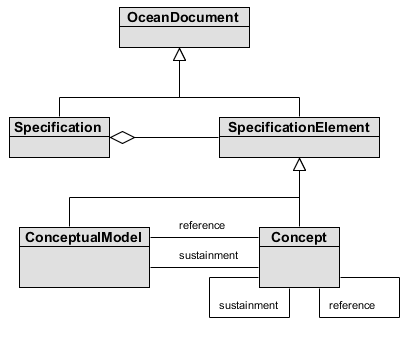
\includegraphics{img/sea_meta_model.png}
	\caption{Meta-modelo do ambiente SEA \cite{silva:00}.}\label{fig:sea_meta_model}
  \end{figure}
  
Com a definição do mapeamento entre os elementos do meta-modelo SEA para o meta-modelo da UML, é necessário uma classe que implemente o algoritmo de
composição: a classe \textit{AspectComposer}. O algoritmo de composição tem duas atividades: \textbf{match} e \textbf{merge}. A primeira atividade
localiza os conceitos selecionados no modelo núcleo pelos pontos de corte ou introduções definidas nos modelos entrecortantes. A atividade de \textit{merge} 
injeta a estrutura ou o comportamento dos modelos entrecortantes no modelo núcleo, fornecendo como resultado um modelo composto. A ferramenta
SEA/Aspect permite a composição automática de diagramas de classe e de sequência.

A composição de diagramas de classe faz uma comparação por nome para selecionar os elementos impactados e tem os seguintes passos:
  
\begin{itemize}
  
	\item \textbf{Comparação e Seleção:} Utiliza uma estratégia que compara diretamente o nome entre aspectos, classes, atributos e métodos. O algoritmo
	procura por elementos que estejam associados com o estereótipo \textit{ClassExtension} nos modelos entrecortantes. Um conceito marcado com este
	estereótipo contém introduções (com o estereótipo \textit{Introduction}) para serem adicionadas em outros conceitos. Essas introduções podem ser a
	adição de campos (métodos ou atributos), mudança na hierarquia de herança ou a implementação de uma interface. 
	
	\item \textbf{Composição:} Quando os conceitos impactados são localizados, o compositor executa uma operação de composição entre os modelos
	entrecortantes e o modelo núcleo. Esta composição produz um modelo composto com os campos, relacionamentos de generalização e realização
	adicionados aos conceitos impactados no modelo núcleo. Esta operação de composição é realizada utilizando o meta-modelo do ambiente SEA, o qual
	permite a adição, remoção e modificação de relacionamentos entre conceitos dinamicamente.

\end{itemize}

A figura \ref{fig:structural_composition_example} apresenta um modelo composto originado pela composição de dois modelos estruturais (diagramas de
classe). O primeiro diagrama é modelado na figura \ref{fig:structural_profile_example} e apresenta o interesse entrecortante que adiciona a
funcionalidade de um objeto ter seu estado copiado para outro objeto utilizando a interface \textit{ICopyable}. O interesse núcleo é modelado pelo diagrama na figura
\ref{fig:structural_core_concern_class_diagram} e modela a estrutura de classes necessária para realizar a reserva de um quarto de hotel. Este
modelo contém a classe \textit{Room} com o método \textit{updateAvailability()} e a classe \textit{ReserveRoomHandler} com o
método \textit{makeReservation()}. O algoritmo de composição de diagrama de classes começa selecionando elementos do modelo núcleo que são
impactados pelos modelos entrecortantes (comparação direta por nome). Neste primeiro filtro, verifica-se que somente a classe \textit{Room} está
presente em ambos os modelos, logo, esta classe pode ter alguma mudança na sua estrutura. Verifica-se que a classe \textit{Room} está marcada com o 
estereótipo \textit{ClassExtension}, o que significa que a mesma sofrerá a introdução de algum membro presente no modelo entrecortante. O próximo
passo do algoritmo é buscar por estereótipos do tipo \textit{Introduction}. Ao executar este passo, seis estereótipos são encontrados, sendo dois
que adicionam um relacionamento de realização de interface entre as classes \textit{Room} e \textit{Reservation} com a nova interface
\textit{ICopyable}, e quatro estereótipos que adicionam os métodos \textit{copy()} e \textit{deepCopy()} nas classes \textit{Room} e
\textit{Reservation}. Neste exemplo de composição, apenas a classe \textit{Room} será modificada pelas introduções do modelo entrecortante. Ao final, 
o modelo composto contém a classe \textit{Room} com dois novos métodos: \textit{copy()} e \textit{deepCopy()} e implementando a interface \textit{ICopyable}. 
A classe \textit{ReserveRoomHandler} não foi modificada com a composição, pois o modelo entrecortante não introduz nenhuma modificação para esta
classe.

  \begin{figure}[!h]
	\centering
	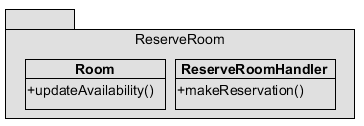
\includegraphics{img/structural_core_concern_class_diagram.png}
	\caption{Modelo núcleo para reserva de quarto.}\label{fig:structural_core_concern_class_diagram}
  \end{figure}
    
  \begin{figure}[!h]
	\centering
	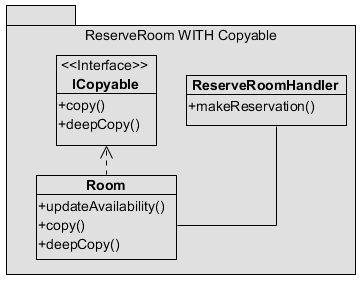
\includegraphics{img/structural_composition_example.png}
	\caption{Composição do modelo núcleo com o modelo entrecortante para cópia de estado entre objetos.}\label{fig:structural_composition_example}
  \end{figure}

A composição de diagramas de sequência realiza a comparação entre conceitos utilizando expressões regulares (\textit{wildcard matching}) e tem os
seguintes passos:
  
	\begin{itemize}
	  
	  \item \textbf{Comparação e Seleção:} Com os modelos núcleo e entrecortantes selecionados pelo desenvolvedor, o algoritmo de composição busca pelos
	  pontos de junção do modelo núcleo que são impactados pelos pontos de corte definidos nos modelos entrecortantes. A busca pode ser separada em três
	  passos:
	  
	  \begin{enumerate}

	    \item \textbf{Obtenção do Ponto de Corte:} Para obter o ponto de corte do diagrama de sequência do interesse entrecortante (modelo
	    entrecortante), o algoritmo busca por invariantes de estado com o estereótipo \textit{AdviceExecutionType}. Este tipo de invariante de estado
	    está associada a um estado que define um ponto de corte.

	    \item \textbf{Separação do Ponto de Corte:} O algoritmo de composição de aspectos utiliza uma expressão regular para separar o ponto de corte em
	    quatro partes: \textbf{tipo de ponte de corte}, \textbf{padrão de tipo de retorno}, \textbf{padrão de identificação} e \textit{padrão de
	    exceção}. O tipo de ponto de corte é mandatório e pode ser um dos tipos suportados pela linguagem AspectJ, os quais incluem \textit{execution},
	    \textit{this}, \textit{target}, \textit{call}, entre outros. O padrão de tipo de retorno é opcional e especifica o tipo de retorno de um ponto de
	    corte. Um método pode retornar um objeto de um determinado tipo, pode não ter nenhum retorno ou pode aceitar qualquer tipo de retorno. O padrão
	    de identificação também é mandatório e contém a assinatura do conceito que deve ser comparada e encontrada no modelo núcleo. Um exemplo de padrão
	    de identificação é a captura de todos os métodos que começam com a palavra \textit{update}. Finalmente, o padrão de exceção é opcional e é
	    utilizado para capturar os pontos de execução os quais lançam exceção de algum tipo especificado pelo padrão.
	    
	    \item \textbf{Comparação e Seleção de Pontos de Junção:} A estratégia de composição utiliza expressões regulares para comparar e selecionar
	    quais pontos de junção são impactados pelos pontos de corte definidos nos modelos entrecortantes. Esta comparação suporta pontos de corte
	    especificados através de \textit{wildcards}, que é uma importante funcionalidade das linguagens para programação orientada a aspectos. O
	    algoritmo começa utilizando o padrão de identificação para encontrar o contexto no qual os conceitos impactados estão envolvidos, como o pacote e
	    a classe de um dado método, por exemplo. Quando todos os conceitos dentro de um dado contexto são capturados, o algoritmo utiliza outra expressão
	    regular para selecionar os nomes dos conceitos capturados. Por exemplo, ao comparar e selecionar um método, o algoritmo verifica o tipo de
	    retorno, os parâmetros (nome, tipo e número de parâmetros) e a assinatura do método. Finalmente, o algoritmo verifica se alguma exceção é
	    lançada. Como saída, os conceitos (classes e métodos) impactados pelos modelos entrecortantes são armazenados para serem usados posteriormente na
	    atividade de composição.
	  \end{enumerate}  
	  
	  \item \textbf{Composição:} Esta etapa compõe os conceitos dos modelos entrecortantes com os conceitos dos modelos núcleo selecionados. O algoritmo
	  recebe como entrada os conceitos impactados do modelo núcleo que devem ser compostos com conceitos dos modelos entrecortantes. O objetivo desta
	  atividade é a injeção de um conjunto de mensagens, linhas de vida, fragmentos combinados e outros elementos do diagrama de sequência no diagrama de
	  sequência núcleo (modelo núcleo), adicionando comportamento definido nos diagramas de sequência dos interesses entrecortantes (modelos
	  entrecortantes). O ambiente SEA facilita a composição de conceitos, como a adição ou remoção de mensagens entre objetos, adição de novos objetos em
	  um diagrama de sequência, etc. O algoritmo de injeção de mensagens entre modelos pode ser separado em dois passos:
	  
		  \begin{enumerate}
		    
		    \item \textbf{Obtenção do Tipo de Execução do Aviso:} Obtém-se o tipo de execução do aviso a partir do valor rotulado da invariante de estado
		    selecionada. Os tipos de aviso suportados são: antes, durante e depois e os mesmos são definidos pelo valor rotulado \textit{adviceType}. O tipo
		    de aviso fornece informações de quando as mensagens serão executadas no diagrama de sequência núcleo.

		  	\item \textbf{Injeção de Mensagens:} Neste momento, o algoritmo já sabe quais são os conceitos impactados, as mensagens a serem injetadas do
		  	modelo entrecortante no modelo núcleo e em qual ponto do tempo as mensagens devem ser injetadas. O próximo passo é a injeção de mensagens e o
		  	reordenamento do diagrama de sequência, pois a injeção de uma mensagem dispara um evento de reordenamento. Com todas as mensagens injetadas e
		  	ordenadas, o algoritmo modifica a cor de fundo de cada mensagem com a cor associada ao respectivo interesse entrecortante, para diferenciar quais
		  	mensagens são provenientes de qual aspecto. A composição produz como saída um diagrama de sequência composto com os conceitos entrecortantes
		  	compostos no diagrama de sequência núcleo.
		  
		  \end{enumerate}
		  
	  \end{itemize}  
	  
\subsubsection{Ordem de Precedência}

A composição de modelos entrecortantes em um modelo núcleo pode gerar diferentes resultados dependendo da ordem de precedência dos interesses. É
possível definir a ordem de precedência entre aspectos utilizando a linguagem AspectJ, com o objetivo de determinar qual aspecto tem precedência
perante outro aspecto ou perante todos os outros aspectos do sistema. Logo, uma abordagem para especificação e modelagem de sistemas orientados a
aspectos deve fornecer uma maneira de tornar determinística a composição de modelos. O problema de precedência ocorre quando em aspectos diferentes,
pontos de corte impactam o mesmo ponto de junção. A linguagem não consegue determinar as mensagens de qual aspecto terão preferência e serão compostas
primeiro. A ordem de precedência envolve os três tipos de aviso: antes, durante ou depois e tem as seguintes regras:

\begin{enumerate}
  \item \textbf{Antes:} Um aspecto com maior precedência executa seus avisos do tipo antes em um ponto de junção antes de outros aspectos com menor
  precedência.
  \item \textbf{Depois:} Um aspecto com maior precedência executa seus avisos do tipo depois em um ponto de junção depois de outros aspectos com menor
  precedência.
  \item \textbf{Durante:} Um aspecto com maior precedência executa seus avisos do tipo durante antes de outros aspectos com menor precedência. Além
  disso, este aspecto tem o controle de permitir a execução de outros avisos ou não.
\end{enumerate}

  \begin{figure}[!h]
	\centering
	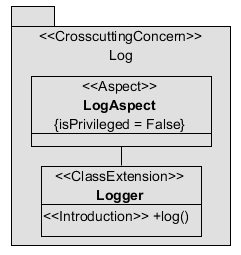
\includegraphics{img/log_aspect.png}
	\caption{Definição da aspecto para registro de mensagens.}\label{fig:log_aspect}
  \end{figure}
  \
  \begin{figure}[!h]
	\centering
	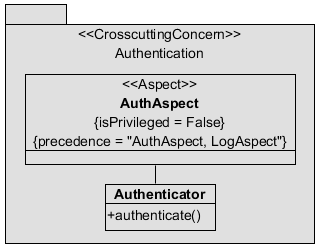
\includegraphics{img/auth_aspect.png}
	\caption{Definição da aspecto para autenticação.}\label{fig:auth_aspect}
  \end{figure}

O Perfil UML proposto por esta dissertação adiciona o valor rotulado \textit{precedence} ao estereótipo \textit{Aspect}. Este valor rotulado define a
ordem de precedência entre aspectos. O tipo deste valor rotulado é um texto, que contém o nome dos aspectos os quais terão a precedência definida.
É possível utilizar expressões regulares na declaração de precedência de aspectos para especificar que um determinado aspecto deve preceder qualquer
outro aspecto do sistema, ou, que um determinado aspecto deve ter menor prioridade do que qualquer outro aspecto. A ordem de precedência é maior da
esquerda para a direita na definição de aspectos. Aspectos com a mesma ordem de precedência, ou sem ordem de precedência definida, serão compostos
seguindo a ordem de especificação dos modelos na modelagem.

A seguir apresenta-se um exemplo de definição de precedência entre dois aspectos: um aspecto para
registro de mensagens (que pode ser visualizado na figura \ref{fig:log_aspect}) e outro aspecto para autenticação de usuário, apresentado 
na figura \ref{fig:auth_aspect}. O aspecto de autenticação de usuário tem maior precedência ao aspecto de registro de mensagens. Para definir essa 
restrição na modelagem, o aspecto de autenticação atribui o valor \textit{'AuthAspect, LogAspect'} ao valor rotulado \textit{precedence}. Esta
definição representa que as modificações estruturais e comportamentais propostas pelo aspecto \textit{AuthAspect} terão precedência perante as 
modificações do aspecto de registor de mensagens \textit{LogAspect}.

\subsubsection{Visualizador de Aspectos}

O perfil UML e o algoritmo de composição implementado na ferramenta SEA/Aspect permitem o intercâmbio de visões de diferentes interesses em
uma modelagem. A visualização do comportamento dos aspectos (interesses entrecortantes) nas funcionalidades núcleo de um sistema facilita a
compreensão e a manutenção de sistemas orientados a aspecto nas primeiras fases de desenvolvimento, permitindo que o desenvolvedor compreenda a ordem de execução do
sistema observando modelos. Um dos obstáculos das abordagens orientadas a aspectos é a dificuldade de compreensão do sistema, já que é difícil
entender o fluxo de execução sem ferramentas adicionais. O visualizador pode ser utilizado na etapa de modelagem, permitindo compreender o sistema em
um mais alto nível de abstração. 

O visualizador de aspectos permite selecionar um interesse núcleo e um conjunto de interesses entrecortantes para serem visualizados em um mesmo
modelo. O objetivo principal deste visualizador é verificar como fica o comportamento do sistema após a adição de um ou mais aspectos. Sem o
auxílio do visualizador, o efeito dos aspectos só pode ser visualizado ao executar o sistema, ou, utilizando ferramentas adicionais para visualização
em nível de código.

\begin{landscape}
  \begin{figure*}[tb]
	\centering
	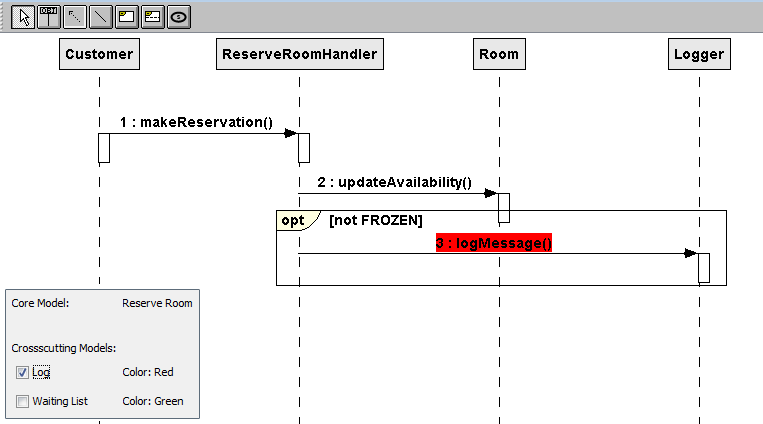
\includegraphics{img/case_study_compound_1.png}
	\caption{Reserva de Quarto Composto com Registro de Mensagens.}\label{fig:case_study_compound_1}
  \end{figure*}
\end{landscape}

A figura \ref{fig:case_study_compound_1} apresenta um modelo composto, que permite a visualização do efeito de um aspecto para registro de mensagens
(\textit{log}) em um interesse para reserva de quartos de um sistema de gerenciamento de hotel. Esta configuração de visões é uma composição
entre o interesse para reserva de quarto e o interesse de registro de mensagens. Observa-se nesta composição que as mensagens do interesse para reserva de 
quartos (\textit{makeReservation()} e \textit{updateAvailability()}) não estão com nenhuma cor de fundo. Já a mensagem do interesse de registro de
mensagens (\textit{log()}) está com o fundo vermelho, pois foi a cor associada a este interesse. Esta diferenciação é importante para diferenciar quais mensagens 
vem de qual interesse no modelo composto. As mensagens que estão com a cor vermelha são provenientes do aspecto para registro de mensagens, logo,
estas mensagens representam o efeito do aspecto no sistema principal. Observa-se um seletor de modelos na parte inferior esquerda do diagrama de
sequência composto. Este seletor permite selecionar quais interesses são visualizados em uma mesma composição. Assim, é possível visualizar o efeito
de um ou mais aspectos ao mesmo tempo. 

O próximo capítulo apresenta dois estudos de caso que detalham a composição e visualização de um ou mais interesses entrecortantes (aspectos) em um
mesmo interesse núcleo.
